%!TEX root = report.tex

\section{Introduction}
%sentiment analysis
Sentiment analysis is one of the important tasks in natural language processing community[8] which helps people navigate the huge amount of user-generated content available online. Machine learning systems that make decision on the attitude of viewpoints to be positive, neutral or negative that enable people to understand the enormous body of opinions on the internet, ranging from product reviews to political positions. 

%challenge
One of the biggest challenges in sentiment analysis, as well as in almost all fields for natural language 
processing research, is the language variation. Words can mean different things to different people, 
and different people express their feeling and idea in a different way. However, such variation is believed
to be tractable from social factors [1]. For example, people of the same ago may speak in a
similar way [12] which might be influenced from their youth education, and people from the same community 
use the same language which is known as jargon. Therefore, social network information provides additional
information to solve the problem in language variable thus improve the general prediction performance
in natural language processing tasks.

%social network
Online social networks provide promising platforms to study the language variations. 
Most online websites have social network behind it, and user-generated content often appears in the context of social media. Therefore nowadays user-relationship information is now more easily obtainable. For example, huge amount of tweets from Twitter express people's opinions on different subjects. Each tweet is associated with a user and users formed social network structure through the mechanisms of ``follower''. When a user forms a link in the network such as Twitter, they tend to have a personal relationship then the principle in language called ``homophily'' suggests that users who are connected via some social relationship may also share similar opinions or linguistic variation (each community may have their own ``jargon'' in expressing ideas and sentiments). Figure 1 from [1] gives an example of how users from different communities may understand the word ``sick'' differently.

\begin{figure}[h]
\centering
\begin{minipage}{.5\textwidth}
  \centering
  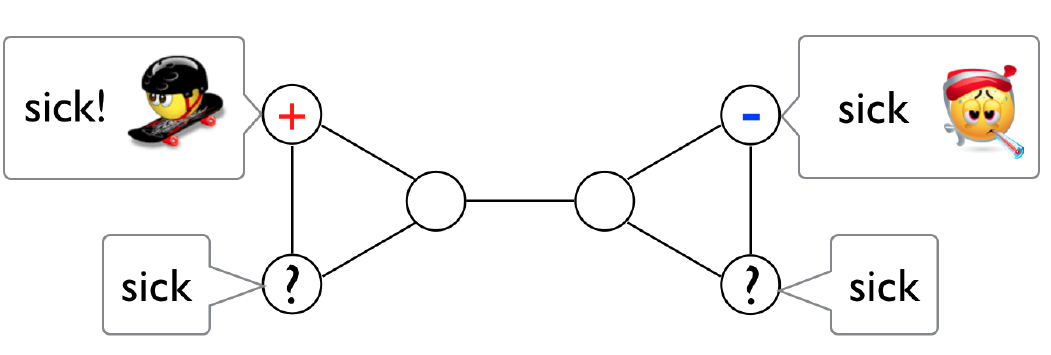
\includegraphics[width=1\linewidth]{sick}
    \label{fig:test1}
\end{minipage}%
\begin{minipage}{.5\textwidth}
  \centering
  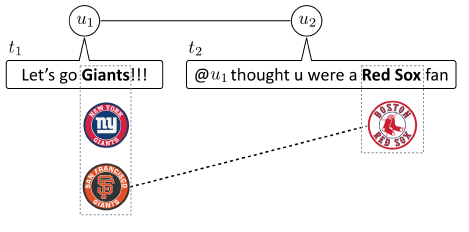
\includegraphics[width=1\linewidth]{Giant}
  
  \label{fig:test2}
\end{minipage}
\caption{Words such as ‘sick’ can express opposite sentiment
polarities depending on the author; Leveraging social relations for entity
disambiguation.}
\end{figure}


Nowadays, models that combine social network information with machine learning classification task are proposed in many literature. However, these models rarely utilize the state-of-art deep learning methods like convolutional neural network or network node embeddings which are common in social network and NLP communities. Previous research either use traditional machine learning methods to incorporate social network structure information as in [7] or they separate the textual and user information to build separate deep learning model as in [8]. None of the previous works directly model the interaction between author information, especially the social network information, and the sentence context. In this paper, we are going to explore different methods that utilize jointly social network information and textual information in sentiment analysis with one joint deep learning model that takes both social network information and textual information as input to classify the sentiment of sentences.

Our paper is structure as follows: section 2 will introduce related work to our task and how we relate them; section 3 will define the problem formally and introduce our dataset; section 4 will introduce our model and intuition; section 5 will demonstrate our numerical result; section 6 will discuss our result and draw our conclusion.
